\documentclass[titlepage]{article}
\usepackage{graphicx} % Required for inserting images
\usepackage[margin=1in]{geometry}  
\usepackage{setspace} 
\doublespacing
\usepackage{booktabs}
\usepackage{amsmath}
\usepackage[utf8]{inputenc}
\usepackage{graphicx}
\graphicspath{{images/}}
\usepackage{float}
\usepackage{ragged2e}
\usepackage{hyperref}
\usepackage{harvard}

\title{Findor et al.(2023) Replication}
\author{Asad Tariq and Isabella Mullen}
\date{\today}

\begin{document}
\begin{titlepage}
    \maketitle
\end{titlepage}

\newpage

\tableofcontents

\newpage

\section{Introduction}
This project replicated Study 3 from \textit{"Equality, Reciprocity, or Need? Mitigating Ethnocentric Bias in Policy Evaluation with  Distributive Fairness"} by Andrej Findora, Matej Hruškab, Roman Hlatkyc, Tomáš Hrustičd, and Zuzana Bošeľováe. The original study examined how different justifications for a social housing project influenced ethnocentric biases in policy opinions. The treatment conditions were three scenarios framed around need, equity, or reciprocity. The reciprocity condition elicited the most support for building the housing project, while the need condition evoked the most disagreement. This was statistically distinguishable from the effects associated with the other conditions (equality and need). This project aimed to replicate Table 3 from the original paper and to explore alternative models fit to the same dependent variable. Replicating Study 3 provided an opportunity to explore how the addition of supplementary covariates changed the analysis.

\justify
The original paper used an ordered logistic regression model to infer the effect of conditional framing of a social housing project on willingness to support the project. We constructed an alternate model that incorporated additional demographic covariates (age, education, sex, and region) to improve the prediction power of the model. When comparing the original and alternate models, the alternate model provides a better in-sample fit and marginally improved out-of-sample predictive accuracy. Incorporating demographic variables highlights additional contextual patterns in the data. Older individuals exhibited stronger support than younger individuals, and there were clear regional differences.

\section{Original Paper}
\subsection{Design Overview: Study 3}
For this project we chose to replicate Study 3 from the original paper (Findor et al. 2023). The experiment was between-subjects with a control group and three treatment conditions (equality, reciprocity, and need). Each participant read a control paragraph describing a fictional village with a Roma settlement where a new apartment building could be built. The scenario explained that the new housing was for the poorest inhabitants of the Roma settlement and that they would be required to pay rent. It also stated that 95\% of the funding came from EU funds, while the remaining 5\% came from the municipality. Participants in the treatment groups were then randomly assigned an additional paragraph corresponding to one of the treatment conditions: equality, reciprocity, or need. In the equality condition, the same amount of money was allocated to projects intended for the non-Roma community. In the reciprocity condition was that only those who worked on the construction of the building could live there. And in the need treatment was that only those who needed the most assistance could live there. After reading the scenarios, participants answered whether they agreed or disagreed with the project on a scale from 1 (“strongly disagree”) to 4 (“strongly agree”). Additional questions were asked but they were not relevant to this replication project.

\justify
The unit of analysis was an individual-level respondent. The sample size for Study 3 consisted of 1,009 survey respondents. This sample was meant to be a nationally representative sample of Slovaks. The original researchers set quotas on gender, age, region, municipality size, and education. The final sample for Study 3 was 52\% female, with a median age of 44.7. The respondents were randomly recruited through an online platform. The survey participants opted in to an online survey, were aware that they were participating in a research study, and were compensated for their time.

\justify
Because this was an online survey, neither we nor the original researchers could verify with complete certainty that each survey was taken independently. However, assuming that each participant needed an account to complete the survey and was exposed to only one randomly assigned condition, it was reasonable to assume independence within the sample. In addition to the randomization of conditions, the relatively large sample size and demographic quotas suggested that the sample was diverse and representative.

\subsection{Methodology}
The original authors used their model to investigate the effects of different framing conditions (equity, reciprocity, and need) on support for redistributive policies in Slovakia. They used ordinal logistic regression to analyze how framing a social housing policy with different distributive fairness principles affected individual support for the policy. They quantified the impact of each framing condition on personal support levels to determine which justifications were the most effective in reducing ethnocentric bias and increasing public support for policies that benefited marginalized groups. This model applied causal inference to assess how changes in the treatment conditions influenced support for the project. This was achieved by randomizing the condition for each participant and comparing responses between groups.

\justify
The authors used this model to explain the dependent variable and treated 'group' as the predictor.

\begin{equation}
\log\left(\frac{P(E3 \leq j)}{P(E3 > j)}\right) = \beta_0 + \beta_1 \text{Equality} + \beta_2 \text{Reciprocity} + \beta_3 \text{Need}
\end{equation}

\begin{equation}
polr(E3 \sim \text{group})
\end{equation}

\justify
The dependent variable in Study 3 was the willingness to support the social housing project, referred to as 'E3' in the data. The dependent variable was an ordinal factor with four levels (1–4). Table 1 presents the descriptive statistics for personal agreement with the social housing policy across four experimental conditions: control, equality, proportionality, and need. The proportionality condition had the highest mean agreement (2.83), while the need condition had the lowest mean (2.40), indicating that respondents were more supportive when fairness was framed around proportional contributions rather than need-based justifications.

\begin{table}[H]
    \centering
    \caption{\textit{Descriptive statistics - Personal agreement}}
    \begin{tabular}{lccccccccccc}  
        \toprule
        \textbf{Group} & \textbf{N} & \textbf{Min} & \textbf{Q1} & \textbf{Median} & \textbf{Q3} & \textbf{Max} & \textbf{Mean} & \textbf{SD} & \textbf{Skew} & \textbf{Kurtosis} \\
        \midrule
        Control        & 252 & 1 & 1 & 3 & 3 & 4 & 2.50 & 1.08 & -0.121 & 1.72 \\
        Equality       & 249 & 1 & 2 & 3 & 3 & 4 & 2.63 & 1.04 & -0.328 & 1.93 \\
        Proportionality & 254 & 1 & 2 & 3 & 4 & 4 & 2.83 & 1.06 & -0.561 & 2.10 \\
        Need          & 254 & 1 & 1 & 3 & 3 & 4 & 2.40 & 1.07 & -0.054 & 1.17 \\
        \bottomrule
    \end{tabular}
\end{table}

\justify
Note: We replicated the results from this table in the original paper (Findor et al. 2023) (Table A19), except for the kurtosis values. We assumed that this discrepancy was due to the use of a different R function or a different definition of kurtosis. Since this value was not relevant to the scope of this project, we left the values as is. The values included in Table 1 are our calculations.

\begin{figure}[H]
    \centering
    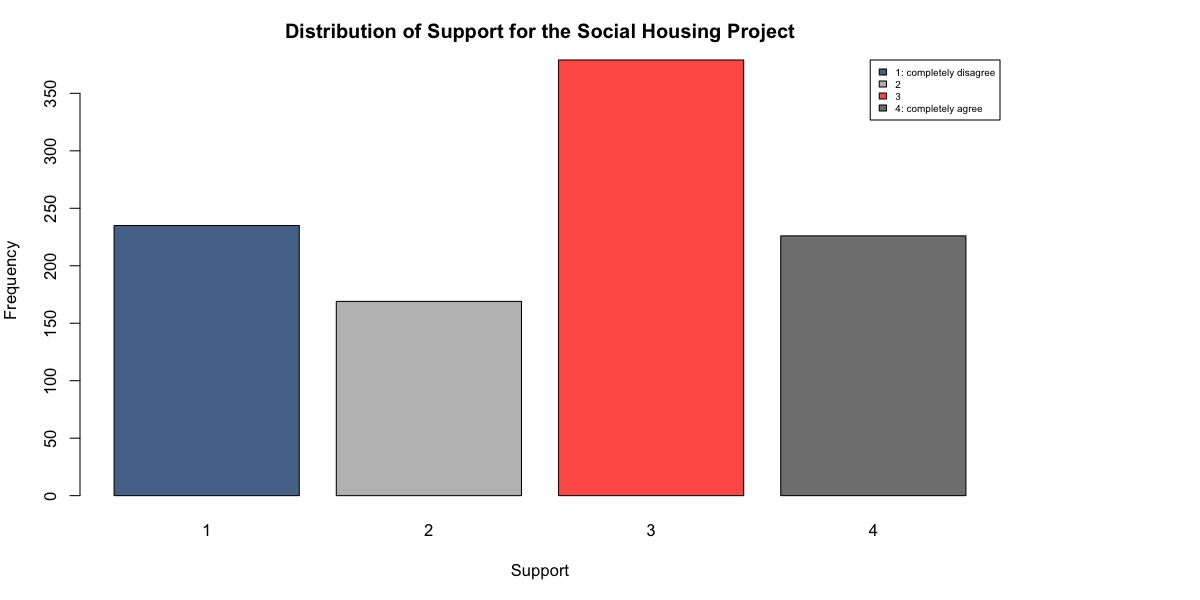
\includegraphics[width=\textwidth]{images/dv_dist.jpeg}
    \caption{Distribution of the Dependent Variable}
    \label{fig:dv}
\end{figure}

\justify
Figure \ref{fig:dv} displayed the overall distribution of the dependent variable for all respondents. The x-axis represented levels of support, ranging from 1 ("completely disagree") to 4 ("completely agree"), while the y-axis represented the frequency of responses. The highest frequency was observed at level 3 ("agree"), followed by levels 1 ("completely disagree") and 4 ("completely agree"), with level 2 being the least common response.

\justify
Figure \ref{fig:dv_group} provided a breakdown of the support for the housing project by condition (control, equality, proportionality, and need). Each bar represented the number of respondents who selected a given level of support, with the colors indicating the experimental group. The proportionality (reciprocity) condition appeared to generate the highest level of support compared to the other groups, while the need frame showed a higher proportion of disagreement than the other conditions. The control and equality conditions displayed relatively balanced distributions.

\begin{figure}[H]
    \centering
    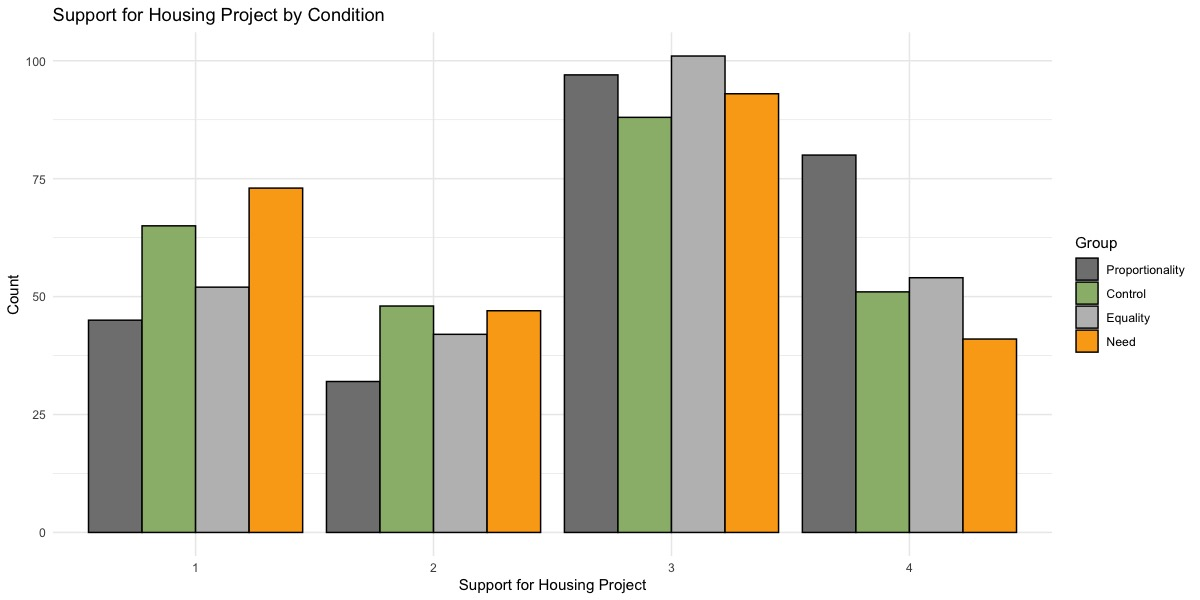
\includegraphics[width=\textwidth]{images/dv_dist_group.jpeg}
    \caption{Distribution of the Dependent Variable by Group}
    \label{fig:dv_group}
\end{figure}

\justify
In the data preparation step, the authors handled missing data by explicitly assigning NA in the income recoding process. The summary statistics code ensured that missing values were ignored, preventing distortions in calculations. However, in the ordinal logistic regression model, missing data was not explicitly handled because there were no missing data.

\subsection{Replication Results}
Table \ref{table:replicationtable} (see on page \pageref{table:replicationtable}) presented the results of an ordinal logistic regression model assessing support for building social housing under different distributive fairness conditions. The control group served as the baseline, with the effects of reciprocity, equality, and need frames estimated relative to it. The results indicated that the reciprocity frame significantly increased support for social housing compared to the control condition, meaning that respondents exposed to this condition were 83\% more likely to express greater support. The equality frame and the need frame did not show statistically significant differences from the control condition. When using reciprocity as the baseline, both the equality and need frames significantly reduced support. The original authors also analyzed the results with the reference category changed to proportionality (reciprocity) rather than control. This did not alter the results but provided a more straightforward interpretation. These findings highlighted how different fairness frameworks influenced attitudes toward redistribution, reinforcing the idea that reciprocity-based narratives resonated more strongly than need-based appeals.

\begin{table}[H]
    \centering
    \caption{\textit{Support for building social housing}}
    \label{table:replicationtable}
    \begin{tabular}{lcccc}
        \toprule
        & Estimate & Std. Error & \textit{p} & OR [95\% CI] \\
        \midrule
        \multicolumn{5}{l}{\textbf{Baseline = Control}} \\
        Reciprocity & 0.60 & 0.16 &  \textless{}.001 & 1.83 [1.33, 2.52] \\
        Equality & 0.22 & 0.16 & .172 & 1.25 [0.91, 1.71] \\
        Need & -0.16 & 0.16 & .323 & 0.85 [0.62, 1.17] \\
        \midrule
        \multicolumn{5}{l}{\textbf{Baseline = Reciprocity}} \\
        Equality & -0.38 & 0.16 & .018 & 0.68 [0.50, 0.94] \\
        Need & -0.76 & 0.16 & \textless{}.001 & 0.47 [0.40, 0.64] \\
        \bottomrule
    \end{tabular}
\end{table}

\justify
Using the original authors' data and the replication code, we successfully reproduced the results of table 3 in the original paper (see table \ref{table:replicationtable}) on page \pageref{table:replicationtable}). Our replication confirmed that the statistical estimates, confidence intervals, and significance levels remained consistent with the published findings. This successful replication supported the robustness of the original analysis and reinforced the conclusions.

\section{Additional Model}
\subsection{Model Design}
After replicating the original model, we constructed an alternate ordered logistic model with a different linear predictor (with more than one independent variable). We chose \textbf{age} (\texttt{AGE}), \textbf{education} (\texttt{EDU}), \textbf{sex} (\texttt{SEX}) and \textbf{region} (\texttt{REG}) along with \texttt{group} (which was already present in the original model) to be part of the alternate model. By including independent variables that related to demographics, we believed that we will have better holistic and contextual predictions of their willingness to support the social housing project.

\justify
The alternate model we considered was the following:
\begin{equation}
polr(E3 \sim group + AGE + EDU + SEX + REG)
\end{equation}

We chose this model for two main reasons: we wanted to determine if the addition of demographic variables would incur a change in the predictions for the dependent variable, and whether a more complex model (with a greater number of predictors) would perform better than a simpler model (with just one predictor).

\justify
See the regression table (Table \ref{table:alterregresstable}) on page \pageref{table:alterregresstable} displays the coefficients and their standard errors for the alternate model.

\subsection{Results}
\subsubsection{In-sample Predictive Performance}
We began by comparing the two models using the Akaike Information Criterion (AIC) and Bayesian Information Criterion (BIC) metrics, the results of which are shown in Table \ref{table:aicbictable} on page \pageref{table:aicbictable}. Using the AIC metric, we observed that the alternative model outperformed the original model, with an AIC value of 2644 compared to 2694 for the original. This indicated that it provides a better fit to the data while balancing the complexity of the model.

\justify
Next, we constructed a calibration plot (Figure \ref{fig:calib_plot}) to compare the prediction probabilities of each model. The calibration plot provided a visual representation of how well the predicted probabilities of two models, 'alter' (red) and 'logit' (blue), align with the observed outcomes for a four-category variable. The 'logit' model was the original model. Each vertical strip on the x-axis corresponded to one of the four observed categories, while the y-axis represents the predicted probability assigned by each model to the observed outcome. Ideally, a well-calibrated model should have assigned high probabilities (close to 1) to the correct category and low probabilities to the incorrect categories.

\justify
The smooth trend lines further highlighted systematic differences between the models. If a model were perfectly calibrated, the probabilities would align closely with the observed outcomes, but the plot suggests systematic miscalibration in both models. The fact that the probabilities did not cluster near 1.0 for the observed outcomes suggested that both models underpredicted the true category probabilities. This may have indicated underlying issues such as class imbalance or overregularization.

\begin{figure}[H]
    \centering
    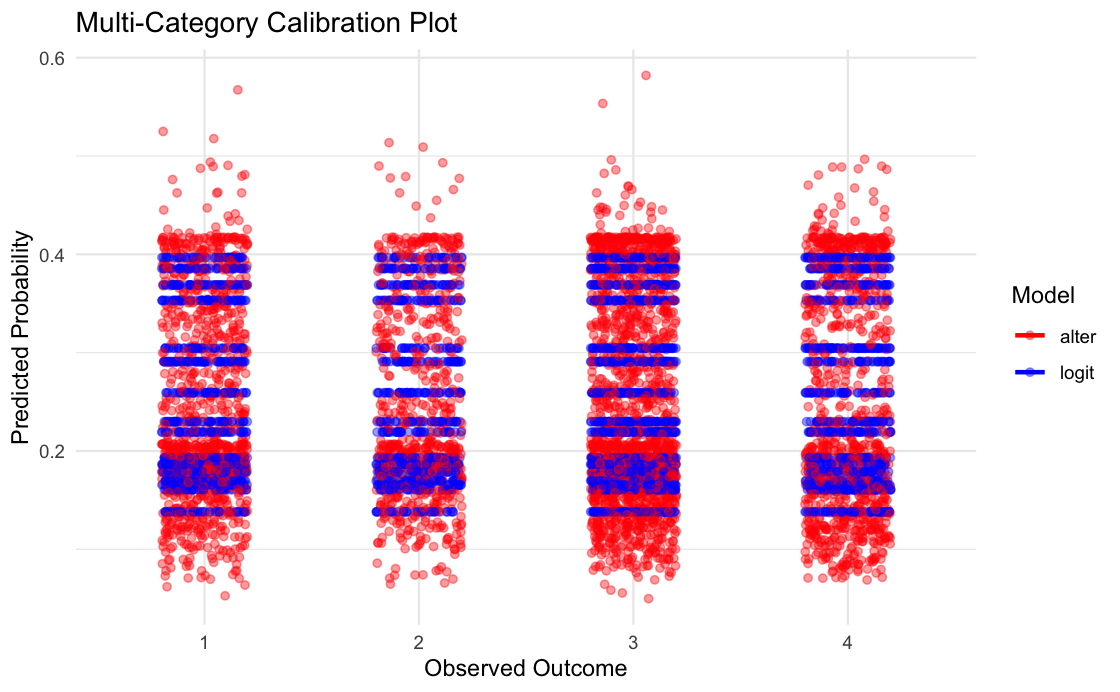
\includegraphics[width=\textwidth]{images/multicategory_calibration.png}
    \caption{A multi-category calibration plot of the predicted probabilities of the two models for each category.}
    \label{fig:calib_plot}
\end{figure}

\justify
We then performed a likelihood ratio test to determine whether our alternate model provided a better fit to the data. The key result (as shown in Table \ref{table:aicbictable}) was an extremely small p-value for the test, $5.3 \times 10^{-12}$, giving us a strong indication that, despite having additional parameters and complexity, the alternate model is significantly better at fitting the data compared to the original.

\justify
Lastly, we plotted the ROC curves to compare the in-sample performance of the two models. Figure \ref{fig:roc_orig} representing the original model, showed ROC curves that closely follow the diagonal reference line. This indicated poor predictive performance. The model’s ability to distinguish between different classes was weak, as the curves did not significantly rise above the diagonal.

\newgeometry{top=1.5cm,bottom=1.5cm}

\begin{figure}[H]
    \centering
    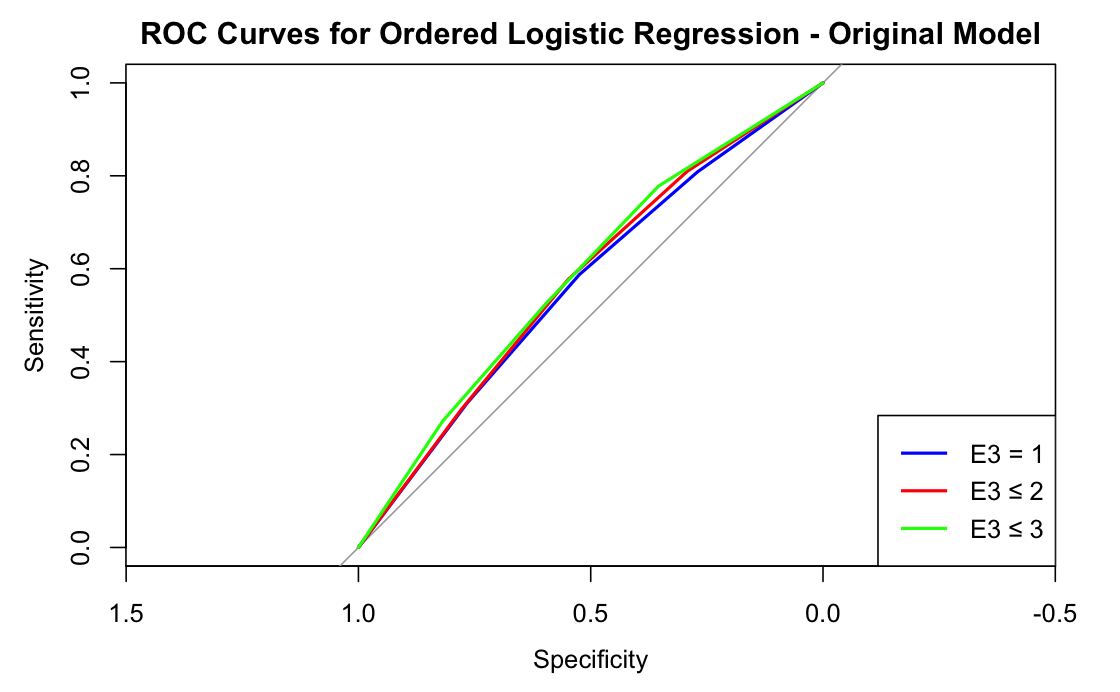
\includegraphics[width=\textwidth]{images/roc_original.png}
    \caption{An ROC plot for the original model.}
    \label{fig:roc_orig}
\end{figure}

\begin{figure}[H]
    \centering
    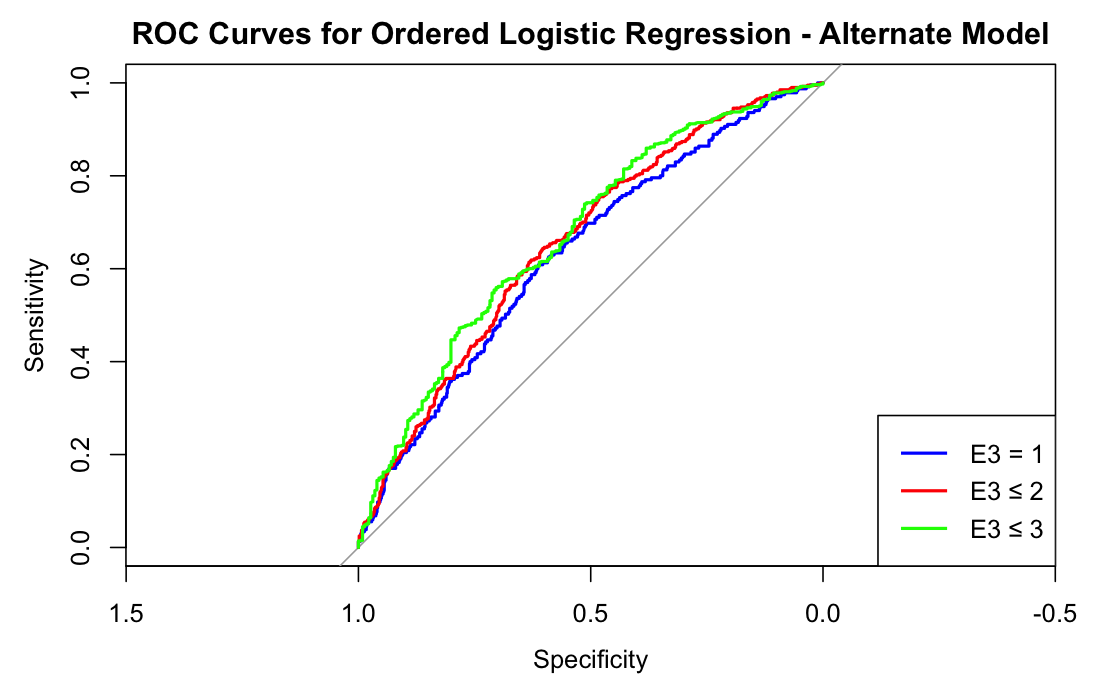
\includegraphics[width=\textwidth]{images/roc_alternate.png}
    \caption{An ROC plot for the alternate model.}
    \label{fig:roc_alter}
\end{figure}

\justify
Comparatively, ROC curves in Figure \ref{fig:roc_alter}, for the alternate model, consistently rose above the diagonal, indicating better sensitivity-specificity trade-offs. This suggested that the alternate model had a stronger discriminatory ability, as its ROC curves are farther from the diagonal and exhibit a greater area under the curve (AUC). The separation between the colored curves for different threshold values of E3 also appeared to be more distinct in the alternate model, suggesting that it provided better differentiation between the ordered categories.

\justify
Overall, the alternate model demonstrated improved classification performance compared to the original model, as indicated by the increased sensitivity and specificity at different threshold levels. This suggested that the modifications made in the alternate model resulted in a better ability to predict the ordered outcomes.

\subsubsection{Out-of-sample Predictive Performance}

To evaluate the out-of-sample predictive performance of the two proportional odds logistic regression models we performed 10-fold cross-validation. To perform cross-validation the dataset was split into 10 equally sized folds (subsets). Each of these folds were used as a test set while the left over 9 folds were used in the training set. This process was repeated 10 times, ensuring that each observation appeared in the test set only once. The aim of both models was to predict the ordinal outcome variable E3, which had four ordered classes (1, 2, 3, 4). The results are shown in Table \ref{tab:cv} below.

\justify
The models were evaluated with each link function on the basis of their accuracy obtained from the cross-validation results. The purpose of checking the accuracy of cross-validation across different link functions was to determine which link function best fits the relationship between the predictor variables and the ordinal outcome (E3). For the original model, the proportion of correctly classified observations remained consistent at $0.376$ across all five link functions: cauchit, cloglog, logistic, loglog, and probit. This indicated that the model was no better than making predictions by randomly guessing. On the other hand, our alternative model showed some improvements over the original, achieving better accuracy with the cloglog link function, which was chosen for the final model, yielding an accuracy of $0.390$.

\begin{table}[!htbp] \centering 
  \caption{Cross-Validation Results} 
  \label{tab:cv} 
\begin{tabular}{@{\extracolsep{5pt}} cccccc} 
\\[-1.8ex]\hline 
\hline \\[-1.8ex] 
 & Model & Method & Accuracy & Kappa \\ 
\hline \\[-1.8ex] 
1 & Original & cauchit & $0.376$ & $0$ \\ 
2 & Original & cloglog & $0.376$ & $0$ \\ 
3 & Original & logistic & $0.376$ & $0$ \\ 
4 & Original & loglog & $0.376$ & $0$ \\ 
5 & Original & probit & $0.376$ & $0$ \\ 
6 & Alternative & cauchit & $0.376$ & $0.052$ \\ 
7 & Alternative & cloglog & $0.390$ & $0.071$ \\ 
8 & Alternative & logistic & $0.375$ & $0.049$ \\ 
9 & Alternative & loglog & $0.372$ & $0.041$ \\ 
10 & Alternative & probit & $0.375$ & $0.047$ \\ 
\hline \\[-1.8ex] 
\end{tabular} 
\end{table}

\subsubsection{Quantity of Interest}

Before building a scenario by manually specifying the predictor values to investigate how one particular independent variable impacted our dependent variable, we wanted to look at how age and region in particular relate to the personal willingness to support the social housing project. 

\justify
Figure \ref{fig:age_effect} illustrated the effect of age on personal willingness to support the social housing project, measured at four levels of willingness (E3 = 1 to 4). Each panel represented a different level of support, with the x-axis showing age, and the y-axis displaying the predicted probability of selecting that level. The solid blue lines represented the estimated effect of age, while the shaded areas indicated confidence intervals.

\begin{figure}[H]
    \centering
    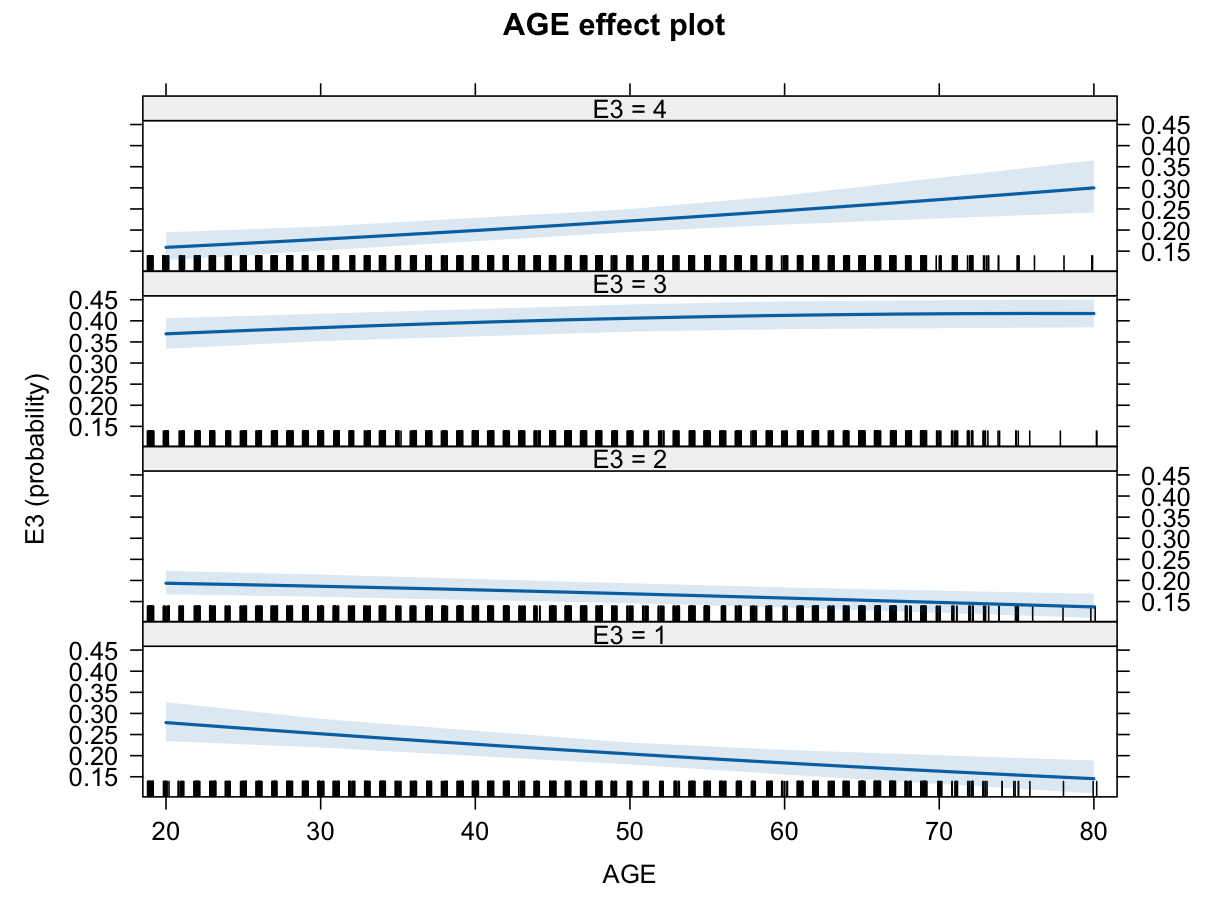
\includegraphics[width=\textwidth]{images/age_effect.png}
    \caption{Effect of the age predictor on the personal willingness to support the social housing project.}
    \label{fig:age_effect}
\end{figure}

\justify
From the figure, we observed that people who were most supportive of the project (E3 = 4) tended to show a slight increase in the probability of support as they aged, suggesting that older individuals were somewhat more likely to express strong support. A similar, though less pronounced, trend was observed for moderate support (E3 = 3), where the probability remained relatively stable, but exhibits a small upward trend with age.

\restoregeometry

\justify
In contrast, for individuals with lower levels of support (E3 = 2 and E3 = 1), the effect of age moves in the opposite direction. The probability of weak support (E3 = 2) decreases slightly with age, while the probability of complete opposition (E3 = 1) shows a more noticeable downward trend, indicating that younger individuals were more likely to express opposition to the project compared to older individuals.

\justify
Figure \ref{fig:reg_effect} presented the estimated effect of region (REG) on personal willingness to support the social housing project (E3), with probabilities plotted across different regional categories. Each panel corresponds to a different level of willingness (E3 = 1 to 4), allowing for a comparative assessment of regional variations in support. The blue dots represent predicted probabilities, while the accompanying orange error bars indicated confidence intervals, reflecting the uncertainty in these estimates.

\begin{figure}[H]
    \centering
    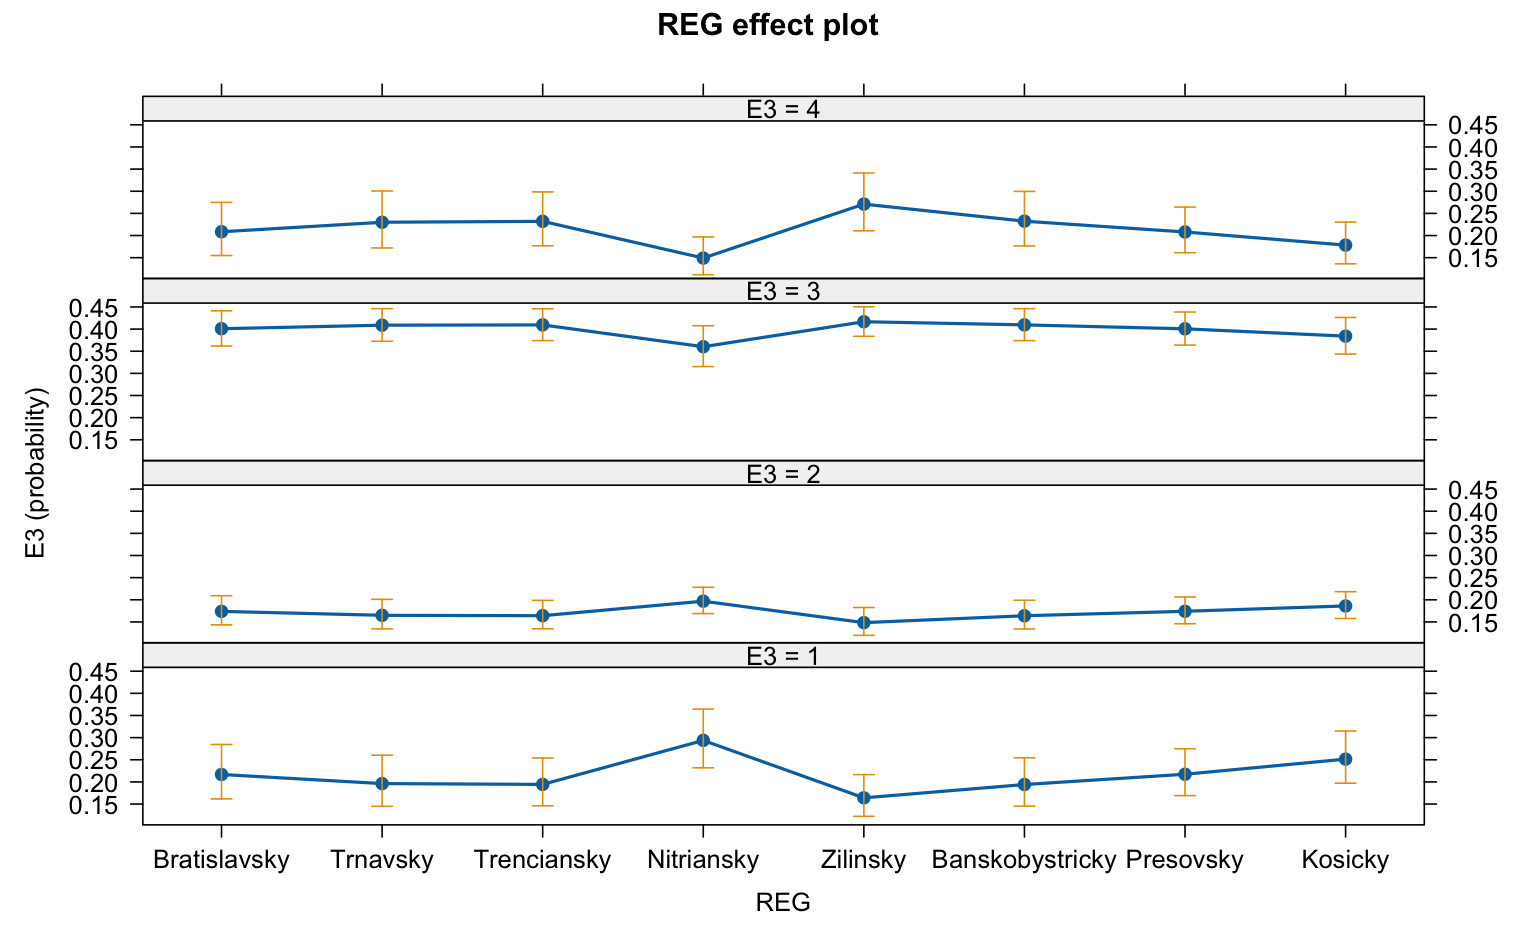
\includegraphics[width=\textwidth]{images/region_effect.png}
    \caption{Effect of the region predictor on the personal willingness to support the social housing project.}
    \label{fig:reg_effect}
\end{figure}

\justify
A clear pattern emerged where the probability of strong support (E3 = 4) fluctuated between regions, with Zilinskii and Nitrianskii exhibiting relatively higher probabilities, while Kosicky demonstrated a lower probability of strong support. In contrast, opposition to the project (E3 = 1) followed an inverse pattern, with higher probabilities observed in Nitriansky and Kosicky, suggesting greater regional resistance to the initiative. The probability of moderate support (E3 = 3) remained largely stable across regions, indicating that regional differences may have exerted a stronger influence on extreme positions (strong support or strong opposition) rather than moderate preferences.

\justify
These findings suggested that regional context played a role in shaping attitudes toward social housing, potentially reflecting underlying socioeconomic, political, or cultural differences across regions. However, the relatively modest variation, coupled with the overlapping confidence intervals, implied that while regional effects were present, they may not have been the dominant factor driving individual support for the project. Further investigation incorporating additional covariates—such as economic conditions, political affiliation, or prior exposure to social housing policies—could have provided a more comprehensive understanding of the mechanisms driving these regional disparities.

\justify
The density plot below (Figure \ref{fig:qoi}) visualized the implied effect of regional differences (Bratislavsky vs. Zilinsky) on personal agreement with the construction of an apartment (E3). The x-axis represented the change in predicted probability of different levels of agreement due to the regional difference, while the y-axis showed the density of these estimated probability shifts.

\begin{figure}[H]
    \centering
    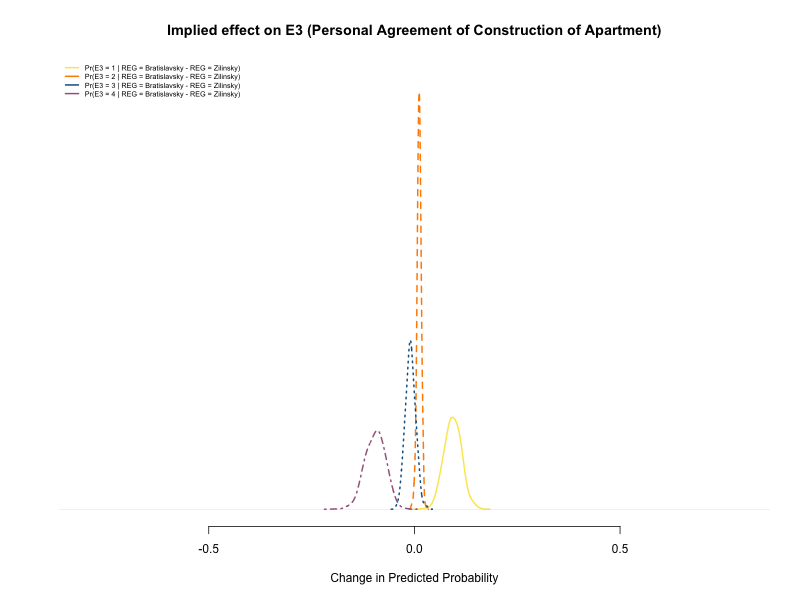
\includegraphics[width=\textwidth, height=10cm]{images/qoi_plot.png}
    \caption{A density plot representing the quantity of interest (region) on personal agreement of Construction of Apartment.}
    \label{fig:qoi}
\end{figure}

\justify
The densities were centered around zero, suggesting that the difference in predicted probabilities between Bratislavsky and Zilinsky was relatively small across all agreement levels. However, E3 = 1 (strong opposition) and E3 = 4 (strong support) exhibited some spread, indicating that regional differences might have had a modest influence on individuals with extreme opinions. Specifically, the density for E3 = 4 (strong support) skewed slightly negative, implying that respondents from Zilinsky might have been less likely to strongly support the construction compared to those from Bratislavsky. Conversely, E3 = 1 (strong opposition) had a slight positive shift, suggesting that opposition could have been somewhat higher in Zilinsky.

\justify
Overall, while the results indicated that regional differences existed, their magnitude appeared limited, as most density curves remained close to zero. This suggested that factors beyond just the region—such as demographic, socioeconomic, or attitudinal variables—were likely playing a more significant role in shaping individual agreement levels.

\subsubsection{Preferred Model}
Based on the in-sample and out-of-sample predictive performance of each model, we concluded that our alternative model performed better at fitting and predicting the data. Additionally, it included demographic predictor variables that provided contextual insight and an advantage over the original model of the authors.

\section{Conclusion}
This replication study of "Equality, Reciprocity, or Need? Mitigating Ethnocentric Bias in Policy Evaluation with Distributive Fairness" successfully reproduced the findings from Study 3, confirming that the reciprocity frame elicited the highest level of support for a social housing project, while the need condition generated the most disagreement. In addition to replicating the original results, this paper introduced an alternate ordered logistic regression model incorporated demographic covariates (age, education, sex, and region) to examine whether these additional factors improved model performance.

\justify
Through a comparison of in-sample and out-of-sample predictive performance using AIC, BIC, and cross-validation, we found that the alternate model provided a better fit to the data, albeit with marginal improvements in predictive accuracy. The inclusion of demographic factors captured additional contextual variation, particularly regarding age and regional differences in support for social housing. Older individuals were more likely to express strong support, while opposition was slightly higher among younger respondents. Regional differences also emerged, although their influence was relatively modest compared to other factors.

\justify
Overall, while the addition of demographic variables improved model performance, the impact of these factors on willingness to support the social housing project was not as pronounced as the influence of framing conditions. These findings suggested that while demographic and regional contexts contribute to shaping public attitudes, framing effects, particularly reciprocity-based narratives, remain the most influential in influencing support for redistributive policies. Future research could further explore the interaction between framing effects and socioeconomic conditions, as well as other attitudinal variables, to provide a more comprehensive understanding of how public support for social policies is shaped.

\subsection{Discussion}
The original authors’ model effectively demonstrates the relationship between willingness to support the social housing project and treatment condition, providing strong evidence for how different fairness principles shape public attitudes toward redistribution. Our reanalysis builds on their work by incorporating additional demographic variables, revealing deeper patterns in the data and improving predictive accuracy. These additions offer valuable insights into the role of individual characteristics in shaping policy support. It is important to note that our replication was limited to Study 3, excluding Studies 1 and 2, which focused on broader fairness perceptions and ethnocentric bias. Given our findings and the original authors’ discussion, we believe that future research should explore how these predictive models could be applied to policy design. Specifically, using these predictions to identify communities most receptive to social housing initiatives could inform targeted interventions, ensuring that policies were framed in ways that maximized public support. Additionally, further cross-cultural research could test whether these framing effects held in different political and social contexts, as suggested in the original study’s conclusions.

\newpage
\section{Appendix}

\begin{table}[!htbp] \centering 
  \caption{Regression Table for Alternate Model} 
  \label{table:alterregresstable}
  \resizebox{9cm}{!}{
\begin{tabular}{@{\extracolsep{5pt}}lc} 
\\[-1.8ex]\hline 
\hline \\[-1.8ex] 
 & \multicolumn{1}{c}{\textit{Dependent variable:}} \\ 
\cline{2-2} 
\\[-1.8ex] & E3 \\ 
\hline \\[-1.8ex] 
 groupEquality & 0.218 \\ 
  & (0.163) \\ 
  & \\ 
 groupProportionality & 0.586$^{***}$ \\ 
  & (0.165) \\ 
  & \\ 
 groupNeed & $-$0.162 \\ 
  & (0.164) \\ 
  & \\ 
 AGE & 0.014$^{***}$ \\ 
  & (0.004) \\ 
  & \\ 
 EDUSecondary (no diploma) & $-$0.493$^{**}$ \\ 
  & (0.219) \\ 
  & \\ 
 EDUSecondary (complete) & 0.222 \\ 
  & (0.221) \\ 
  & \\ 
 EDUUniversity & 0.471$^{*}$ \\ 
  & (0.242) \\ 
  & \\ 
 SEXFemale & $-$0.075 \\ 
  & (0.119) \\ 
  & \\ 
 REGTrnavsky & 0.126 \\ 
  & (0.254) \\ 
  & \\ 
 REGTrenciansky & 0.138 \\ 
  & (0.245) \\ 
  & \\ 
 REGNitriansky & $-$0.407$^{*}$ \\ 
  & (0.238) \\ 
  & \\ 
 REGZilinsky & 0.344 \\ 
  & (0.242) \\ 
  & \\ 
 REGBanskobystricky & 0.139 \\ 
  & (0.245) \\ 
  & \\ 
 REGPresovsky & $-$0.003 \\ 
  & (0.233) \\ 
  & \\ 
 REGKosicky & $-$0.193 \\ 
  & (0.234) \\ 
  & \\ 
\hline \\[-1.8ex] 
Observations & 1,009 \\ 
\hline 
\hline \\[-1.8ex] 
\textit{Note:}  & \multicolumn{1}{r}{$^{*}$p$<$0.1; $^{**}$p$<$0.05; $^{***}$p$<$0.01} \\ 
\end{tabular}}
\end{table}

\begin{table}[!htbp] \centering 
  \caption{Log likelihood, AIC, and BIC comparison between the Original and Alternate Model} 
  \label{table:aicbictable}
  \resizebox{10cm}{!} {
\begin{tabular}{@{\extracolsep{5pt}}lcc} 
\\[-1.8ex]\hline 
\hline \\[-1.8ex] 
 & \multicolumn{2}{c}{\textit{Dependent variable:}} \\ 
\cline{2-3} 
\\[-1.8ex] & \multicolumn{2}{c}{E3} \\ 
\\[-1.8ex] & (1) & (2)\\ 
\hline \\[-1.8ex] 
 groupEquality & 0.220 & 0.218 \\ 
  & (0.161) & (0.163) \\ 
  & & \\ 
 groupProportionality & 0.604$^{***}$ & 0.586$^{***}$ \\ 
  & (0.163) & (0.165) \\ 
  & & \\ 
 groupNeed & $-$0.159 & $-$0.162 \\ 
  & (0.160) & (0.164) \\ 
  & & \\ 
 AGE &  & 0.014$^{***}$ \\ 
  &  & (0.004) \\ 
  & & \\ 
 EDUSecondary (no diploma) &  & $-$0.493$^{**}$ \\ 
  &  & (0.219) \\ 
  & & \\ 
 EDUSecondary (complete) &  & 0.222 \\ 
  &  & (0.221) \\ 
  & & \\ 
 EDUUniversity &  & 0.471$^{*}$ \\ 
  &  & (0.242) \\ 
  & & \\ 
 SEXFemale &  & $-$0.075 \\ 
  &  & (0.119) \\ 
  & & \\ 
 REGTrnavsky &  & 0.126 \\ 
  &  & (0.254) \\ 
  & & \\ 
 REGTrenciansky &  & 0.138 \\ 
  &  & (0.245) \\ 
  & & \\ 
 REGNitriansky &  & $-$0.407$^{*}$ \\ 
  &  & (0.238) \\ 
  & & \\ 
 REGZilinsky &  & 0.344 \\ 
  &  & (0.242) \\ 
  & & \\ 
 REGBanskobystricky &  & 0.139 \\ 
  &  & (0.245) \\ 
  & & \\ 
 REGPresovsky &  & $-$0.003 \\ 
  &  & (0.233) \\ 
  & & \\ 
 REGKosicky &  & $-$0.193 \\ 
  &  & (0.234) \\ 
  & & \\ 
\hline \\[-1.8ex] 
Log-Likelihood & -1341.27 & -1304.2 (0.0000000000533) \\ 
Observations & 1,009 & 1,009 \\ 
Akaike Inf. Crit. & 2,694.000 & 2,644.000 \\ 
Bayesian Inf. Crit. & 2,724.000 & 2,733.000 \\ 
\hline 
\hline \\[-1.8ex] 
\textit{Note:}  & \multicolumn{2}{r}{$^{*}$p$<$0.1; $^{**}$p$<$0.05; $^{***}$p$<$0.01} \\ 
\end{tabular}}
\end{table} 

\justify
We used ChatGPT 4o LLM/AI tool in this report. We used this tool to understand the author's original code. We also used ChatGPT to save time debugging our code, helping with latex formatting, and translating some of the original materials from Slovak to English. The tool was helpful and efficient for these tasks. ChatGPT was also used to help interpret the calibration plot and ROC curves we made for the in-sample predictive performance of the two models. It helped us understand how the models performed for in-sample predictions compared to each other.

\justify
Please click \href{https://chatgpt.com/share/67d47a4f-e0d8-8004-8a43-8cba73891e43}{here} \href{https://chatgpt.com/share/67d4a1ab-f9f4-8012-8bf6-c9248ddeb44c}{and here} to view the conversations we had with ChatGPT.

\section*{References}

Findor, Andrej, Matej Hruška, Roman Hlatky, Tomáš Hrustič, and Zuzana Bošeľová. 2023. “Equality, Reciprocity, or Need? Bolstering Welfare Policy Support for Marginalized Groups with Distributive Fairness.” American Political Science Review 117(3): 805–21. doi:10.1017/S0003055422001046.

\end{document}